\section{Lexicon}
\label{sec:lexicon}

\begin{description}

	\item[Bloom's taxonomy:] set of hierarchical models useful to
		classify learning objectives into levels of complexity and
		specificity. The models capture these different levels in
		different domains - namely cognitive, affective and sensory.
		For engineering and natural sciences purposes the most
		important is likely the cognitive one, whose levels are
		reported in Table~\ref{tab:blooms-taxonomy};

		\begin{table}[!htbp]
			\centering
			\begin{tabular}{|llp{0.7\textwidth}|}
				\hline
				1 & \emph{Remember} & be able to recognize
				or remember facts, terms, basic concepts, or
				answers without necessarily understanding
				what they mean \\
				2 & \emph{Understand} & be able to organize,
				compare, translate, interpret, give
				descriptions, and state the main ideas \\
				3 & \emph{Apply} & be able to use prior
				knowledge to solve problems, identify
				connections and relationships and how they
				apply in new situations \\
				4 & \emph{Analyze} & be able to break
				information into component parts, determine
				how the parts relate to one another,
				identify motives or causes, make inferences,
				and find evidence to support generalizations
				\\
				5 & \emph{Evaluate} & be able to present and
				defend opinions by making judgments about
				information, the validity of ideas, or
				quality of work based on a set of criteria
				\\
				6 & \emph{Create} & be able to build a
				structure or pattern from diverse elements
				and to put parts together to form a whole \\
				\hline
			\end{tabular}
			\caption{Summary of the knowledge levels defined in
			Bloom's taxonomy~\cite{bloom1956taxonomy}.}
			\label{tab:blooms-taxonomy}
		\end{table}

	\item[\acfp{ILO}:] what students should know or be able to do at the
		end of the course that they couldn't do before. They should
		be about students performance. Typical verbs used to
		describe \acp{ILO} are: ``Memorize, identify, recognize,
		define, find, classify, describe, list, discuss, select,
		compute, analyse, explain, compare, construct, review,
		solve, prove,'' etc;

	\item[\acfp{KC}:] acquirable units of cognitive functions. They can
		be facts, concepts, procedures, etc. Importantly, a \ac{KC}
		must have the quality that it is possible to design tests
		that can show whether a student has acquired that \ac{KC} or
		not. \emph{If one defines something for which one cannot
		test whether a student acquired that thing or not, then that
		thing is not a \ac{KC}.} Specially important cases of
		\acp{KC} in engineering and natural sciences education are
		\emph{facts}, \emph{procedures} and \emph{concepts}. These
		correspond to mental representations, abstract objects or
		abilities that make up the fundamental building blocks of
		thoughts and beliefs, plus instructions, recipes, or sets of
		commands that show how to achieve some result, such as to
		prepare or make something;

	\item[\ac{SOLO} taxonomy:] a taxonomy that describes levels of
		increasing complexity in students' understanding of
		subjects. In practice, a way of classifying educational
		learning objectives into levels of complexity and
		specificity. A graphical illustration of the SOLO taxonomy
		is given in Figure~\ref{fig:SOLO-taxonomy}. A video
		explaining what the levels mean using LEGOs as an example
		can be found searching ''SOLO taxonomy using LEGO'' in
		youtube.

		\begin{figure}[!htbp]
			\centering
			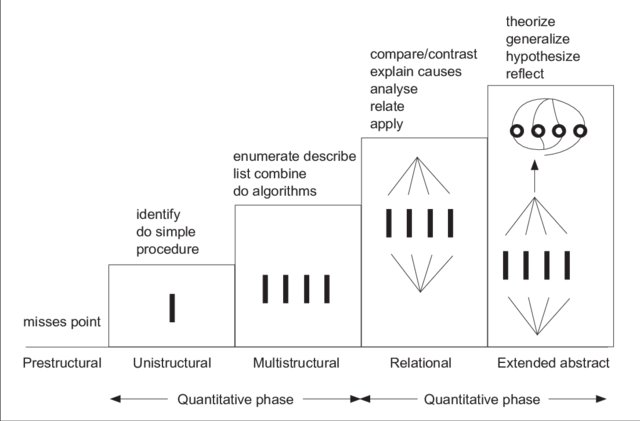
\includegraphics[width = 0.8\textwidth]{SOLO-Taxonomy}
			\caption{Graphical representation of the \ac{SOLO}
			taxonomy as proposed in~\cite{biggs1982evaluation}.}
			\label{fig:SOLO-taxonomy}
		\end{figure}

	\item[taxonomy:] (i.e., a set of ordered labels) 

	\item[\acfp{TLA}:] the work that is done in and out of the class in
		relation to the course, e.g., seminars, lectures, labs, etc.
		See
		\url{https://www.uwc.ac.za/TandL/Pages/TandL-Activities.aspx}
		for some more examples; 

\end{description} 

